\chapter{Near Detector Beamline Measurements}
\label{ch:nd-blm}

%\fixme{Starting from the fall 2012 CDR content; Geoff is preparing update}

\section{Introduction}
\label{sec:nd-blm-intro}

This chapter outlines the DUNE strategy for measurements of secondary
beam particles in the region behind the beam absorber. 
Those measurements are designed to provide constraints 
on the neutrino flux at the near and far
detectors, and data on the pulse-to-pulse variation
of the beam for beam diagnostic purposes. A description of equipment
for monitoring the proton beam's interaction with the proton target
can be found in Volume 2: The Beamline at the Near Site. 

The measurements and apparatus described in this chapter fall into
the category of equipment designed specifically for DUNE to
detect muons exiting the decay tunnel. 

\section{Design Considerations}
\label{sec:nd-blm-design}

\subsection{General}
The requirements for the beamline measurements, 
as discussed in the NDC requirements documentation~\cite{nd_requirements_doc}, \fixme{old LBNE reference}
are intimately related to how well the neutrino flux must be known. 
Given that DUNE does not have the luxury to construct identical 
Near and Far Detectors, a near-far comparison is more complicated than it was in
the MINOS experiment~\cite{gnumi-validation}, for example.   
While external hadron-production measurements can place strong 
constraints on the pion and kaon production in the target, they do not 
provide any confirmation of the simulation of other key features, such 
as the horn focusing, secondary interactions, and the 
pion scattering and absorption in the air-filled decay volume. 

In addition to the external measurements, covered in Section~\ref{ch:ext-meas}, 
that confirm the simulation of the thick target, horn material, decay tunnel and
absorber, it is desirable to constrain the flux by making independent
measurements at the 4--5\% level of the muons that penetrate the absorber. It would not be practical to do this for all penetrating muons, but sufficient measurements at a few positions can be done in a  cost-effective way. 

\subsection{Muon Measurements}
\label{subsec:nd-blm-muon-meas}
The dominant, two-body decays of pions and kaons that produce
neutrinos also result in the creation of daughter muons. Monitoring
the muons exiting the decay volume can provide information about the
direction, size, shape and flux of the neutrino beam.  The daughter
muon and neutrino energies in those two-body decays are completely
anti-correlated. For example, a $\pi^+\rightarrow \mu^+\nu_\mu$
decay will result in a $\nu_\mu$ with an energy, $E_\nu$, between
zero and 0.43$E_\pi$ plus a $\mu^+$ with an energy of 
$E_\mu=E_\pi-E_\nu$ between 0.57$E_\pi$ and $E_\pi$. This has the
effect that the muon takes 79\% of the pion energy on average,  
leaving the neutrino with only  21\%. Thus, on average, the
muon energy is 3.75 times that of the neutrino.

The primary physics goal of DUNE is to measure the transmutation
of $\nu_\mu$s to $\nu_e$s over the 1300km between Fermilab
and the far detector site.
Therefore it is essential for DUNE to cross-check the estimate of 
background $\nu_e$s present in the beam by using several
methods to measure their rates at the Fermilab site. 
There are two dominant sources of $\nu_e$s present in the
neutrino beam, muon decays and kaon decays. 
The muon systems are designed to directly measure the 
muons that penetrate absorber with an energy 
threshold as low as possible, i.e. directly measure those muons 
whose decays are a major source of background $\nu_e$s, . 
A measurement of the spectrum of those muons will translate
 directly into constraints on the spectrum of background $\nu_e$s.
That constraint has the enormous advantage of being independent of poorly understood 
neutrino-nucleus cross sections.

Because muons and neutrinos come from the same parent pion and kaon
decays, a measurement of the absolute muon flux in conjunction with the energy spectrum
seen in the muon monitors can constrain the absolute neutrino flux.  
The goal for the DUNE muon monitors is to determine the absolute muon flux
to an accuracy of 5\% above a muon energy of 6~GeV (which corresponds to
a neutrino energy of 1.6~GeV) in the central part of the absorber.
Figure~\ref{fig:nu_mumon_frac} shows the total simulated neutrino flux at the 
Far Detector overlaid with the flux from only neutrinos having pion or kaon parents that contribute to the signal
seen in the muon monitor.  The simulation shows that between 3~GeV and 10~GeV, more than 90\% of 
the neutrinos in the Far Detector come from this subset.

\begin{cdrfigure}[Simulated neutrino fluxes at Far Detector]{nu_mumon_frac}
{The total simulated neutrino flux at the Far Detector (black solid) overlaid with the neutrino flux, also at the Far Detector, coming from neutrinos with pion or kaon parents that contribute to the muon-monitor signal (red dashed), averaged over the back of the absorber. As shown in Figure \ref{fig:AbsorberThickness}, the muon systems will probe down to 1.5 GeV in neutrino energy on the beam axis.}
\includegraphics[width=3in,angle=0]{nu_muon_fraction}
\end{cdrfigure}

\begin{cdrfigure}[Ratio of the flux on-axis to the flux 0.4~mrad off-axis]{fluxRatio}
{Ratio of the neutrino flux on-axis to the flux 0.4 mrad off-axis at the Far
Detector position.}
\includegraphics[width=4in,angle=0]{fluxRatio}
\end{cdrfigure}

It is essential to monitor the stability of the beam direction over
time. Figure~\ref{fig:fluxRatio} shows the effect on the muon-neutrino
flux in the Far Detectors when the beam is misaligned by 0.4~mrad.  
For example, above 6~GeV, the ratio of the Far Detector flux over 
the Near Detector flux changes by 2\%.  
To keep the change in the neutrino beam less than 1\% in all energy bins,
the beam direction must be known to a precision of approximately 0.2~mrad. 
Because the muon monitors will be located approximately 275~m
from the beam target, this requires a measurement of the muons to an
accuracy of approximately 5~cm.

The rate of muons crossing the monitors will be quite high, with
preliminary LBNF beam simulations suggesting approximately 50 million
muons per cm$^{2}$ for a pulse of $10^{14}$ protons-on-target. The
muon monitors must also be capable of operating in a high-radiation
environment.  For example, the expected dose in the area downstream of
the NuMI absorber is as high as 100~MRad per year \cite{ref:NuMIBeamMonitors}.

%
%
%%%%%%%%%%%%%%%%%%%%%%%%%%%%%%%%%%%%%%%%%%%%%%%%%%%%%%%
\section{Muon-Measurement Facilities}
\label{sec:nd-blm-muon-measurement-facilities}

The muon measurements are carried out in the region immediately
following the hadron absorber at the end of the decay tunnel, below
the Absorber Service Building (LBNF 30).  A view
of the absorber area and the muon alcove is shown in Figure~\ref{fig:AbsorberPerspectiveOverview}. 
The axis of the decay pipe cuts across the muon alcove at an angle, and the size of the alcove
is largely determined by the requirement that it contain the
shadow of the four-meter-diameter decay pipe, projected through the
alcove, as shown in the elevation view of Figure~\ref{fig:AbsorberElevationView}. 

Figure~\ref{fig:AbsorberPerspectiveOverview2} shows the downstream side of the
absorber and a conceptual layout of the muon systems described in various sections of this
chapter.  
The absorber itself is encased in concrete. The first set of
muon-measurement devices, from left to right, is a
set of three variable-pressure gas Cherenkov counters, which are
mounted directly to the rear wall of the absorber. Following that is an
array of diamond ionization detectors and finally a set of stopped-muon 
counters which are interspersed between walls of
steel ``blue blocks''.   The blue blocks are there to provide several
depths at which to monitor the stopped muons as they range out in the
material. A second array of ionization devices will also be placed farther downstream within the blue blocks.


\begin{cdrfigure}[The Absorber Hall elevation view]{AbsorberPerspectiveOverview}
{The Absorber Hall overview. The Absorber Service Building (LBNF 30) is on the surface and allows for crane access to the Absorber Hall. The muon alcove is directly behind the absorber. }
\includegraphics[width=3in,angle=0]{AbsorberPerspectiveOverview}
\end{cdrfigure}

A perspective view of LBNF 30 is shown in Figure~\ref{fig:AbsorberPerspectiveOverview2}, 
and a detail of the lower level of Absorber Hall
is given in Figure~\ref{fig:AbsorberElevationView}.  The HV, water systems 
and gas systems for the muon monitors will be located nearby on the lower level.
The readout electronics will be located in racks close to the surface. 

\begin{cdrfigure}[The Absorber Hall]{AbsorberPerspectiveOverview2}{A perspective view of the Absorber Hall area.}
\includegraphics[width=6in,angle=0]{AbsorberPerspectiveOverview2}
\end{cdrfigure}

It is important to have precise knowledge of the amount of material muons pass
through before they are registered in the muon systems. The absorber
itself is a complex, heterogeneous assembly of various materials. 
Figure~\ref{fig:AbsorberElevationView} show the absorber conceptual 
design (more detail is available in Volume 2 of this CDR). A hole
in the front side of the absorber, at left, is both surrounded and followed by the
aluminum core of the absorber. The core is then surrounded by steel 
and standard steel ``blue blocks'', 
which are in turn surrounded by concrete.  This
complex geometry must be carefully understood and simulated in order
to make the muon measurements effective. 


\begin{cdrfigure}[Absorber conceptual design, elevation view]{AbsorberElevationView}
{Absorber conceptual design. The figure shows the elevation view of the 
absorber at the end of the decay tunnel. The beam axis is shown by
the blue line. The absorber is constructed of several different 
materials as shown: aluminum core in blue and grey, concrete 
(grey and tan), and steel (in brown and green).}
\includegraphics[width=6in,angle=0]{AbsorberElevationView}
\end{cdrfigure}

Figure~\ref{fig:AbsorberThickness} shows the energy lost by a
horizontal muon as it traverses the absorber, as a function of the
distance from the beam axis along a 45$^\circ$ line perpendicular to the beam axis. 
In the central region, roughly to a distance of  105~cm, the muons lose between 5.0 to 6.4~GeV, so that the
lowest-energy muons leaving the absorber at that point correspond to
neutrino energies of $\sim$ 1.5 to 2.0~GeV. At a radius of roughly 105~cm, the
full thickness of steel causes the muons 10~GeV or more,
corresponding to neutrino energies of $\sim$ 2.6~GeV. From the
perspective of the muon systems it will be desirable to lower these
thresholds if possible. This might be accomplished by using more
aluminum in the front part of the absorber or by judiciously locating detectors inside the 
absorber material. 

\begin{cdrfigure}[Energy loss in absorber]{AbsorberThickness}{The energy loss a muon, parallel to the beam axis, experiences as it traverses the material in the absorber. The muon's energy loss is plotted versus the distance from the beam axis, along a 45 $^\circ$ line perpendicular to the beam axis. Muons suffer between 4.7 and 9.3~GeV of energy loss depending upon where they cross the absorber.}
\includegraphics[width=5in,angle=0]{AbsorberThickness}
\end{cdrfigure}

%
%
%%%%%%%%%%%%%%%%%%%%%%%%%%%%%%%%%%%%%%%%%%%%%%%%%%%%%%%
\section{Muon Cherenkov Detectors} % (WBS 130.03.03.04)}
\label{sec:nd-blm-muon-cherenkov}

\subsection{Introduction}

A Cherenkov variable-pressure, gas Cherenkov counter, operated in differential mode
will be deployed downstream of the absorber.  The counter will be mounted on a movable 
stand that will allow the system to scan in a plane transverse to the beam axis. 
The Cherenkov counter deployed by DUNE will not image individual Cherenkov rings, but rather will see the
integrated signal from many muons due to the very large instantaneous flux. 
In addition, by varying the radiator gas pressure, and hence the 
Cherenkov threshold, the system's index of refraction will vary, 
allowing it to map out the muon momentum distribution.

Figure~\ref{fig:MuonBeta} shows the expected distribution of
velocities, $\beta$ ($v/c$), for muons and electrons after exiting the
absorber. 
Figure~\ref{fig:MuonAngle} shows the expected angle with respect to the beam for
electrons and muons with similar velocities (implying that both are visible above the 
same Cherenkov threshold).  Despite the similar velocities, the muons are much more likely
than the electrons to be directed parallel to the beam.

Therefore, a detector that takes advantage of the directional nature of Cherenkov
light will have less background contributions from electrons and other isotropic 
background particles such as neutrons, than will an ionization system, for example. 

\begin{cdrfigure}[Simulated electron and muon velocities upon exiting absorber]{MuonBeta}
{Simulated electron and muon velocities exiting the absorber. This plot is based on a 
simulation gnumi\cite{GNuMI} of the LBNF beamline.}
\includegraphics[width=4in,angle=0]{MuonBeta}
\end{cdrfigure}


\begin{cdrfigure}[Simulated electron and muon angles upon exiting absorber]{MuonAngle}{lSimulated plot of angle with respect to the beam for 
electrons and muons exiting the absorber.
This plot is based on a gnumi simulation of the LBNF beamline.}
\includegraphics[width=4in,angle=0]{MuonAngle}
\end{cdrfigure}


\subsection{Reference Design}

The simple Cherenkov counter design
employs a gas radiator contained in a pressurized tube. The very forward
Cherenkov light in a narrow cone of $\pm$ 1 mrad is collected at the end of the tube
by a mirror that reflects the light 90 degrees towards a photosensor
located outside the high-radiation field of the muon beam. The gas
pressure, varied from vacuum to twenty atmospheres, will determine
the index of refraction, and hence the Cherenkov angle versus muon-momentum. 
Several such tubes will be constructed in an array
transverse to the beam direction. The resulting pressure scan will
give the momentum distribution of the muons at an array of points
across the end of the absorber.  

Figure~\ref{fig:CherenkovCounterDetail} shows how the
Cherenkov system will be constructed. Safety considerations suggest that the
diameter of the radiator tube and light-guide tube be six inches
or less.  A 
photosensor, located outside the direct radiation field of the muons, will
view the primary mirror through a telescopic optical system.

\begin{cdrfigure}[[Cherenkov counter design]{CherenkovCounterDetail}
{The Cherenkov counter prototype design. 
Muons at threshold momentum emit forward Cherenkov light which is
reflected via one flat mirror 45 degrees) to a PMT located outside of the muon
radiation field.}
\includegraphics[width=6in,angle=0]{CherenkovCounterDetail}
\end{cdrfigure}

The preferred option is to use a gas Cherenkov system containing a
noble gas with a high index of refraction, where the density of the
gas can be varied to change the Cherenkov threshold. The noble gas
will reduce potential degradation due to reactivity in the high
radiation field of the post-absorber environment. Varying the pressure
will provide more information about the momentum spectrum of the
muons.

The combination of a flat mirror and a 90$^0$ mirror will reflect
light out to a PMT. The UV-sensitive PMT will collect light from
normal incidence on the primary mirror with a 2~mrad acceptance, the light
yield per particle will be approximately one photon near
threshold. That is more than ample light for the system where the
particle flux is of order 10$^7$ per cm$^2$ through the radiator section. 


\subsection{Prototype Development and Testing}
\label{subsec:nd-blm-muon-cherenkov-proto}

A prototype Cherenkov counter, along with associated fully automated gas systems,
HV systems, and data acquisition system has been constructed and is undergoing
testing in the NuMI neutrino beam's muon alcove 2. In addition, three diamond
detectors~\cite{ref:CERNdiamond} for ionization measurements have also been installed into the alcove.
Figure~\ref{fig:Alcove2Cherenkov} shows the prototype detectors in NuMI alcove 2.

The counter has an automated gas system with a settable pressure that ranges
from vacuum to 20 atm, corresponding to muon Cherenkov thresholds of 
200 GeV/c and 1 GeV/c respectively. When operated at vacuum, the PMT registers all background light
unrelated to the gas, e.g. transition radiation, light from particles hitting the window and PMT glass.
Those contributions are observed to be very small relative to the coherent, directional Cherenkov light.

The counter is constructed with a 1 meter long radiator section
as shown in Figure~\ref{fig:CherenkovCounterDetail} . A 20 foot extension allows the reflected 
Cherenkov light to travel to a sapphire pressure window viewed by a photo multiplier tube.

The prototype is now fully integrated into NuMI operations and real-time waveforms can be viewed online as shown in Figure~\ref{fig:MuonDetectorWaveforms}. The top panel shows the waveform from the Cherenkov counter at 2 atm gas pressure, that corresponds to a muon momentum threshold of 3 GeV/c. The second panel shows the waveform from a $9mm\ \times\ 9mm$ diamond detector mounted to the front flange of the Cherenkov radiator section as shown in the inset 
of Figure~\ref{fig:Alcove2Cherenkov}.

The extracted NuMI proton beam, Resistive Wall Monitor (RWM) signal 
is also recorded with an identical digitizer. That allows a direct, bucket-by-bucket (individual proton pulses) 
comparison of the proton current onto the NuMI primary proton target, and the muons measured after the absorber with a 400ps time resolution.

\begin{cdrfigure}[Muon gas Cherenkov counter]{Alcove2Cherenkov}{A prototype muon gas Cherenkov detector for DUNE.  
Muons travel through an L-shaped 4" Conflat pipe filled with a pressurized gas. A flat mirror mirrors directs the optical photons to a photo multiplier. The lower right inset shows the 20 bar MKS pressure reading achieved by the Cherenkov gas system, and the inset on the upper right shows the CERN/Cividec diamond detectors mounted to the Cherenkov housing.}
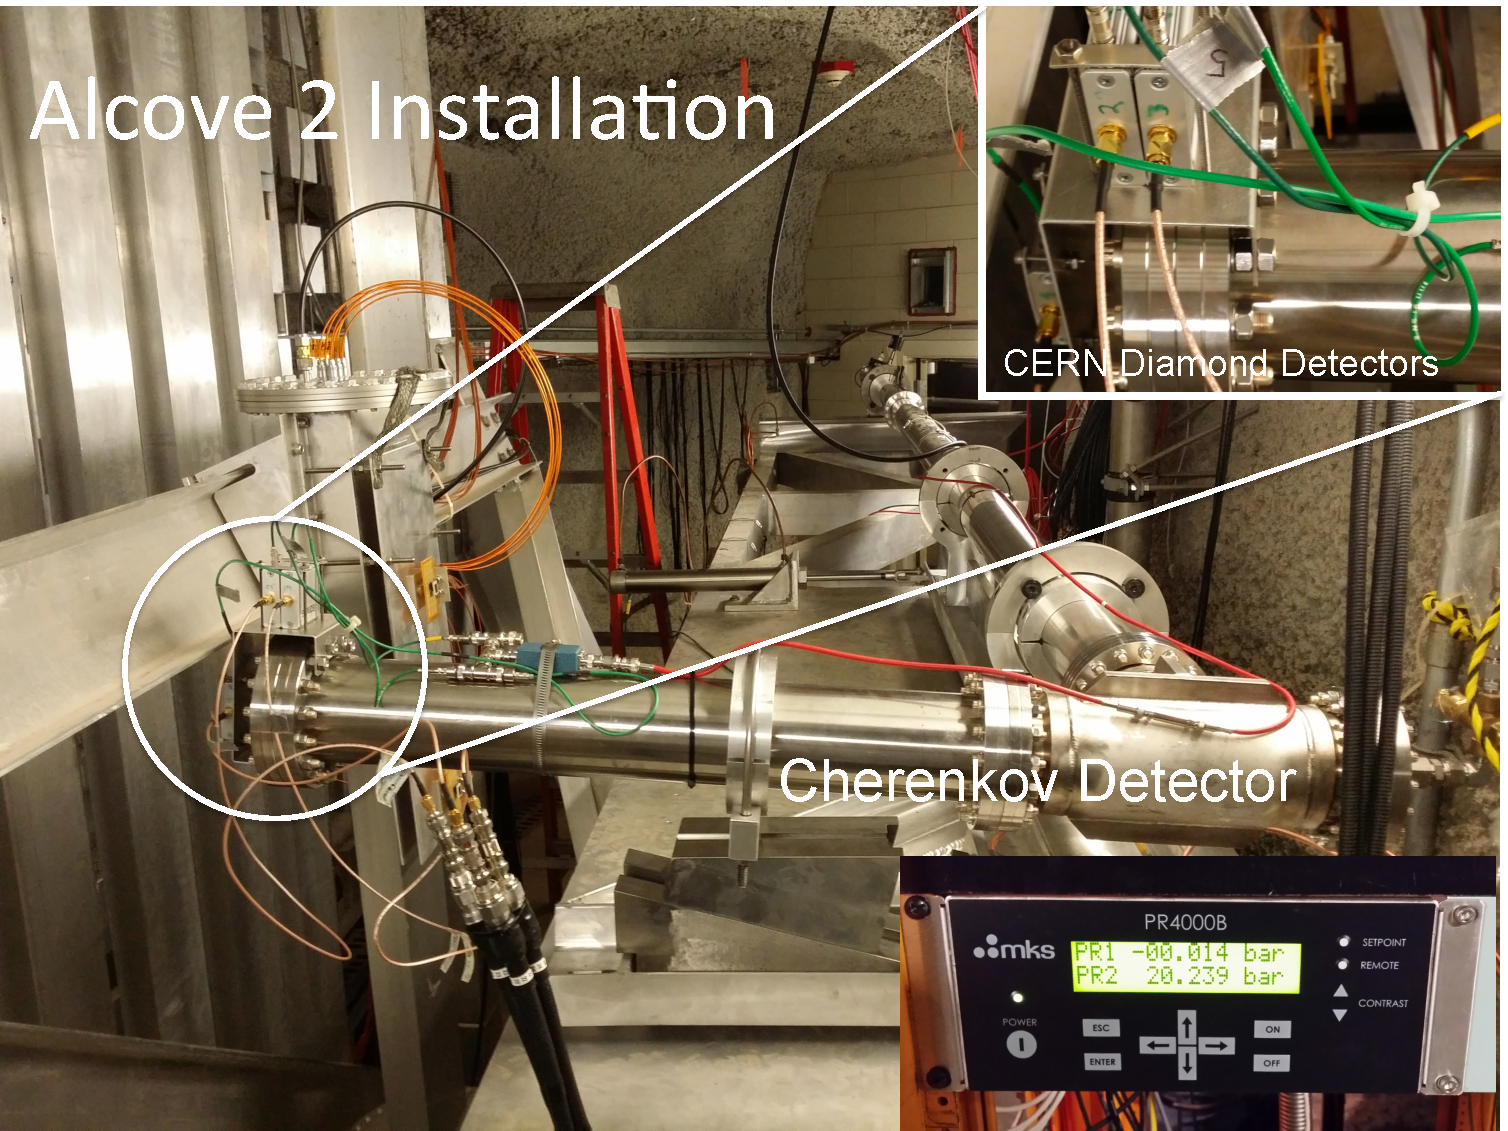
\includegraphics[width=5.5in]{Alcove2Cherenkov}
\end{cdrfigure}

\begin{cdrfigure}[Muon gas Cherenkov counter]{MuonDetectorWaveforms}{The realtime display of the
muon detector prototypes in operation on the NuMI beam line. The top two panels are the Cherenkov counter and CERN diamond detector \cite{ref:CERNdiamond}, The signals are transmitted through low-loss heliax cable, and then the waveform is digitized at 2.5 GHz with a 12 bit dynamic range, and the recorded onto disk storage for analysis. The signal from the muons is contained in the short beam pulse "buckets" created by the accelerator RF structure. The fast timing allows the prompt muon signal to be easily separated from potential backgrounds such as stopped muon decays, beta decays, and neutrons.}
\includegraphics[width=5in]{MuonDetectorWaveforms}
\end{cdrfigure}

A second set of muon detectors, the final DUNE design, are being constructed at this time (2015). They are being installed directly behind the NuMI proton beam dump (muon alcove 1). They will be mounted on a movable stand, and the entire setup will be eventually transferred the DUNE absorber hall. The higher radiation environment of alcove 1 will be more similar to the eventual DUNE installation. It will allow the DUNE muon detectors to be calibrated in the NuMI beam and ready for use in the DUNE beam.
\subsection{Installation}

Installation will begin following the absorber installation and the installation of the stopped muon systems
systems. The counters will be removed from the NuMI Alcove 1 area after calibration in the NuMI beam, and then 
stored until they are needed for DUNE. 
The gas handling system will be located nearby, also on the lower level of the Absorber Hall.

\subsection{Operation}

Because the system will be located in a radiation-controlled
environment that will not be accessible during beam operation, it is
essential that the electronics and gas handling system be both robust
and remotely operable.  The prototype system in use at the NuMI area can be relocated for that purpose,
or if desired a new system may be constructed.
Periodic access will be required to the utilities area to replace gas bottles.

%
%
%%%%%%%%%%%%%%%%%%%%%%%%%%%%%%%%%%%%%%%%%%%%%%%%%%%%%%%
\
\section{Muon-Ionization Measurements}
\label{sec:nd-blm-muon-ionization}

\subsection{Introduction}

Post-absorber muon measurements in most of the recent neutrino-beam
experiments have typically employed a planar array of ionization
counters to measure the muon profile and intensity. The 
NuMI beamline~\cite{ref:NuMIBeamMonitors} and the K2K~\cite{ref:K2K}~\cite{ref:Maruyama}
and T2K~\cite{ref:T2KMuIon}~\cite{ref:T2KMuMon} experiments have all
utilized parallel-plate ionization detectors. These counters have been
shown to work in the high-radiation environment. 

K2K and T2K have also deployed solid-state silicon detectors~\cite{ref:Maruyama}
\cite{ref:RD42A}. The advantage of silicon is that it is less
sensitive to changes in the air temperature and pressure. However, these %solid-state 
sensors are not as radiation-tolerant as the parallel-plate ionization 
chambers and will only be used in T2K for the initial
beam operation. 

DUNE is however in the process of evaluating CVD diamond detectors
as ionization measurement devices. Their advantage is two-fold, they are much more
radiation resistant than silicon, and they provide a much faster signal than ion chambers
which allows them to distinguish between background and the prompt muon signal. They 
are also very stable and require no gas system.

The DUNE NDC plans to use the ionization devices, e.g. CVD diamond, to monitor
the beam stability, direction and shape, 
and also potentially to determine the absolute flux of muons or to determine the 
muon-energy spectrum. Instead, the stopped-muon counters %(WBS 130.03.03.02) 
and gas Cherenkov detector %(WBS 130.03.03.04) 
will be used, respectively, to determine the flux and energy
spectrum of the muons. 

\subsection{Reference Design}

The reference conceptual design is to use CVD diamond ionization detectors arranged in two
arrays. Each array will measure the centroid of the muon beam to insure a stable neutrino flux
at the near and far detectors. The detectors are arranged in a diamond shaped arrays as shown in 
Figure~\ref{fig:AbsorberPerspectiveOverview2} and Figure~\ref{fig:CherenkovStandView}.

\begin{cdrfigure}[Model of ionization detector layout]{CherenkovStandView}{A model of the ionization detector layout behind the Cherenkov detector stand showing the 13 detectors in a grid configuration.}
\includegraphics[width=3in,angle=0]{CherenkovStandView}

\end{cdrfigure}

\begin{cdrfigure}[Model of ionization detector array]{DiamondArrray}{A model of one the two ionization detector arrays
that measure the muon flux and muon beam centroid.
}
\includegraphics[width=3in,angle=0]{DiamondArray}
\end{cdrfigure}

The reference design for DUNE includes two layers of ionization counters, one 
behind the absorber and a second one behind steel shielding blocks. 
DUNE wants to achieve a precision in the beam center of 0.2~milliradians
(5~cm for a 250~m decay pipe). A quick study has 
determined the sensitivity for various arrangements of the ionization counters for each layer and
Figure~\ref{fig:cross} shows the typical precision such a system can achieve.
DUNE design was motivated by a desire to use a grid array with some of the 
counters removed, and still achieve the desired sensitivity, 
thus reducing the total number of needed counters.

\begin{cdrfigure}[ionization detector performance for cross-with-corners layout]{cross}{Precision as a function of detector width for a cross-shaped detector 
with assumed 5\% random calibration offsets.}
\includegraphics[width=70mm]{cross}
\end{cdrfigure}

Several different designs for the counter arrangement were studied and the
area covered by the detectors was varied. A toy Monte Carlo model was
developed to estimate the precision of each design. The muon profile
was assumed to be a Gaussian with a spread of 130~cm in the $x$ and $y$
dimensions and a center at the origin. 
The standard deviation on the beam center was studied as a
function of array coverage for several designs and for 2\%, 5\% and
10\% random systematic error offsets. Figure~\ref{fig:cross} shows the
precision of the detector array as a function of the width of the
detector cross arrangement of the detectors.

The results show that the width of the detector array affects the
precision more than the layout of the detectors. Increasing the array
size improves the precision greatly. 

The DUNE muon ionization detector design consists of two arrays of 
ionization counters, which is motivated by the NuMI target experience.  Over a period of several months, the number of events per proton on target gradually decreased over time, especially in the energy range from 2-4 GeV.  
This reduction in neutrino flux is attributed to 
target radiation damage.  Figure~\ref{fig:numi_mumon_ratio} shows the ratio of the signal seen  in the first muon alcove to the signal seen in the second muon alcove versus time.  This ratio decreased in a similar manner over time.  
The first alcove was immediately after the absorber, while the second alcove was behind approximately 12 m of rock, and therefore saw only higher energy muons, since the lower energy ones would range out before reaching the second alcove.  
This gradual decrease in the ratio of the signals seen in these arrays was an indication of the target degradation and the relative reduction in the 
low-energy part of the neutrino and muon fluxes.  \footnote{Similar trends were seen in the ratios of the other muon alcove signals, but the first/second ratio saw the largest effect.}

It will be necessary to be able to monitor this ratio in DUNE on a spill-by-spill basis to look for signs of target degradation or horn failure.  
Therefore, a second ionization array, placed behind several layers of 
shielding blocks, will be necessary.  In Figure~\ref{fig:AbsorberPerspectiveOverview2}
the second array is placed behind 4 m of steel shielding.  Since the density of steel is roughly 3 times larger than that of rock, this is comparable to the depth of the NuMI second muon alcove, which sits behind 12 m of rock.  More detailed studies will need to be performed to determine if this is the optimal location for sensitivity to changes in the target density.


\subsection{Prototype Design and Testing}

The prototype testing of the diamond detectors is described above in the 
Cherenkov counter section, Section~\ref{subsec:nd-blm-muon-cherenkov-proto}.
For the DUNE ionization detectors, a small array of prototype
counters will be built and operated in the existing NuMI
alcove 1 to determine the optimal design and operating conditions for
the DUNE monitors. This will be done in 2016 and 2017. 
It will provide a good field test in roughly the same environment as expected during DUNE
operations. It will also be cross-checked against the existing NuMI
muon-monitoring system.  The goals of these tests are to understand the linearity of the response of these counters (by comparing the observed signal to variations in the beam intensity), their long-term stability and operational reliability.  

\subsection{Installation}

The system installation will begin following completion of the
Absorber Hall and LBNF 30 and the installation of the stopped-muon counter system
(described in Section~\ref{sec:nd-blm-stopped-mu}).

\subsection{Operation}

The muon-monitor-system data will be displayed in the control room 
at the Absorber Hall upper level on
a spill-by-spill basis to monitor the beam stability and look for potential signs of target or horn degradation. 
This control room will be accessible during the beam operation.
The data will also be displayed at central run control.  

%
%
%%%%%%%%%%%%%%%%%%%%%%%%%%%%%%%%%%%%%%%%%%%%%%%%%%%%%%%
\section{Stopped-Muon Detector} % (WBS 130.03.03.02)}
\label{sec:nd-blm-stopped-mu}

\subsection{Introduction}

The second system under development is stopped-muon counters, also called
Michel-electron detectors. This method will measure the muon flux without
suffering from some of the disadvantages intrinsic to systems that
detect through-going muons. The strategy employed here is to stop muons
in a material with significant carbon content 
and, via muon capture, to produce $^{12}B$ that will in turn undergo $\beta$ decay.
 The high-carbon material, in this case graphite, surrounds a Cherenkov radiator
material which is sensitive to electrons from muon decay or 
high-energy beta decays.  Figure~\ref{fig:StoppedMuonCounterDetail} 
shows the conceptual design of a single stopped-muon counter. 


\begin{cdrfigure}[Michel-electron detector conceptualization]{StoppedMuonCounterDetail}{Conceptual design of a single Michel-electron detector (stopped-muon counter)}
\includegraphics[width=5in,angle=0]{StoppedMuonCounterDetail}
\end{cdrfigure}

The detectors will only operate in the lower-rate
environment that is present many microseconds after the beam pulse is
over. There are two possible modes for this type of system. 
The first is an integrating mode where the characteristic decay time of 
2.2~$\mu s$ for muon decay and corresponding beta-decay lifetimes is used to
unfold the total number of decays. The other mode under
investigation uses the ability to record individual decays rather
than an analog current measurement. This mode may allow a more precise absolute
normalization of the flux and fit the muon lifetime in the Michel-electron detector. 
This will provide a more robust cross-check on the
muon signal than will ionization detectors, which are sensitive to delta
rays, photon conversions and other charged particles.

Although this technique has never been tried on a large scale, a small
demonstration project in K2K was able to see Michel decays with a
$10^{3}$ signal/background ratio and to measure the absolute rate with
30\% precision\cite{ref:K2KMuDecayMon}.

\subsection{Reference Design}

The stopped-muon detector reference design
is modular and based on a Cherenkov radiator of
minimum size to contain a 52.8-MeV electron and distinguish it cleanly
from lower-energy radioactivity. This conceptual design employs
a liquid mineral oil  radiator. The radiator will be coupled to four photomultiplier tubes (PMT) or
other photon counter.  The entire module will be surrounded by a 
liquid scintillator veto layer, and the entire module then
encased in a material that provides both a uniform-density stopping
target for muons and some shielding from incoming neutrons. One or two
signal channels will be associated with each module, and the full
waveform from each channel over approximately 100~ms will be recorded
on each beam pulse.

Nine modules will be placed just behind the absorber in a cross pattern.  An additional 12 will be 
placed at multiple depths in the shielding in order to sample the muon flux
from different energies, as shown in Figures~\ref{fig:AbsorberElevationView2}. 
The shielding will simultaneously act to range out the muons and shield the detectors from 
neutrons. The Cherenkov light from Michel-decay electrons will exit the 
counter and be collected by either nearby PMTs or by a light guide which will
guide the light to a remote optical sensor.  

\begin{cdrfigure}[Absorber conceptual design, elevation view]{AbsorberElevationView2}
{Stopped muon counter conceptual design. The figure shows the elevation view of the 
absorber at the end of the decay tunnel along with the locations of a subset of the
stopped muon counters, and showing a possible arrangement of ``blue blocks'' 
and stopped muon detectors. In this case there is roughly 2~GeV of energy loss 
per wall of blue blocks. The final arrangement is under investigation and will depend on the
final absorber design.}
\includegraphics[width=6in,angle=0]{AbsorberElevationView2}
\end{cdrfigure}

To probe the muon flux at lower energies, it may also
be feasible and/or desirable to place some additional modules within
the downstream part of the absorber or in the outermost radii of the
decay-pipe shielding. The ability to do this may be limited, however,
by the presence of muons from stopped, positively charged pion decays
due to nearby hadron showers.

Besides the Michel decays of stopped muons, the system will
independently measure both the $\mu ^{+}$ and $\mu ^{-}$ stopped
rates as a function of depth. 
While the 2.2~$\mu $s decay time of the $\mu^+$ is a reliable
signature, in mineral oil roughly 8.5\% of the $\mu^{-}$ undergo capture
on the $^{12}C$ nucleus, and 15\% of those leave behind a $^{12}B$
ground state nucleus. That $^{12}B$ nucleus will undergo $\beta$ decay
with a half-life of 20.20~ms and an electron spectrum with an endpoint
of 13~MeV. This signal is expected to yield a reliable measurement of the rate of stopped
$\mu^{-}$.

\subsection{Prototype Development and Testing}

Prototype development activity for the Michel-electron detectors will
be divided into studies of the rate and radiation environment where
the detectors will be located and development of the counters
themselves.

The radiation environment will be studied both with Monte Carlo 
simulations and by measurements from initial prototype detectors 
in the NuMI muon alcoves \cite{ref:NuMIBeamMonitors}.
The prototypes will be installed into the alcoves in 2016 and 2017.
Studies will be performed to determine if the photon sensors
can survive the radiation environment at the location of the Michel
detector. If the sensors can survive, they can be attached directly to
the Cherenkov medium; if not, optical guides will have to bring the
light to a lower-radiation area to the side of the beam. Potential
radiation damage to the Cherenkov radiator itself will also be
studied.

The detector design will focus on selecting radiator and shielding
material, photon-detection technology and control/readout
hardware. Possible radiators include aerogel, which may be designed to
be replaced periodically, and flowing liquids such as H$_2$O or
mineral oil. Long-timescale saturation from the very high-rate
environment of the beam spill could affect the photon-counting devices
\cite{ref:HighRateCounting}. Thus, it will likely be necessary to
design fast-switching, high-voltage circuits that turn on the photon
counters in the first few microseconds after the spill is over. A
similar system was developed in the 1990s for the Brookhaven Muon
(g-2) Experiment~\cite{ref:G2} .

\subsection{Installation}

The stopped-muon counters will be installed after completion of the 
Absorber Hall and LBNF 30  
and installation of the absorber. 
They will be placed into the spaces between the blue-block walls on
support frames.   There will be access to the areas between the shield blocks 
from the side, and the stopped-muon counters will be designed so that they can 
be wheeled in from the side.  If needed, they could then be moved around to measure
the stopped-muon rates across the muon beam.

\subsection{Operation}

The muon-monitor-system data will be displayed in the control room on
a spill-by-spill basis to monitor the beam stability. Because the
system will be located in a radiation-controlled environment that will
not be accessible during the beam operation, it is essential that the
electronics be designed for remote operation.

